% concatenated from main.tex
\documentclass[reqno, 11pt]{amsart}
\usepackage[letterpaper, margin=1in]{geometry}
\usepackage[utf8]{inputenc} 
\usepackage[T1]{fontenc} 
\usepackage{amsmath}
\usepackage{amsthm} 
\usepackage{amssymb}
\usepackage{tikz}
\usepackage[colorlinks=true, allcolors=black]{hyperref}
\usepackage[nameinlink]{cleveref}

\newtheorem{theorem}{Theorem}
\theoremstyle{definition}
\newtheorem{lemma}{Lemma}
\newtheorem{definition}{Definition}
\newtheorem{remark}{Remark}
\newtheorem{proposition}{Proposition}
\newtheorem{corollary}{Corollary}


\newcommand{\abs}[1]{\left\lvert#1\right\rvert}
\newcommand{\norm}[1]{\left\lVert#1\right\rVert}
\newcommand{\sqb}[1]{\left[ #1 \right]}
\newcommand{\dd}{\mathrm{d}}
\newcommand{\II}[1]{\mathbf{1}{#1}}


\author{Saba Lepsveridze}
\address{Department of Mathematics, Massachusetts Institute of Technology}
\email{sabal@mit.edu}

\author{Oriol Solé-Pi}
\address{Department of Mathematics, Massachusetts Institute of Technology}
\email{oriolsp@mit.edu}


\begin{document}

\title{Uniform Geodesic Drawings of Graphs}
\begin{abstract}
We study crossing numbers of dense graph drawings whose vertices are uniformly distributed either on the unit sphere or in a compact convex planar domain.  We prove a sharp inequality for weighted geodesic drawings on $\mathbb S^2$ in a continuous setting: among all measurable edge arrangements of a fixed density, the amount of crossings is minimized by connecting pairs of points within a fixed distance threshold.  We also prove a planar analogue for straight-line drawings in convex planar domains. We transfer these continuous results to finite graphs using a smoothing argument. In the small density limit, we recover the conjectured midrange crossing constant lower bound of $8/(9\pi^2)$ for this restricted model.
\end{abstract}

\maketitle


\section{Introduction}\label{sec:intro}
A \textit{drawing} of a graph $G$ is a representation of the graph on either $\mathbb R^2$ or $\mathbb S^2$ in which the vertices are represented by distinct points and the edges by continuous simple curves connecting their respective endpoints. A drawing is called \textit{good} if no edge contains a vertex in its relative interior, no two edges are tangent to each other or intersect at infinitely many points, and no three edges share an interior point. A \textit{crossing} is a point which lies at the intersection of two edges but does not represent a vertex. The crossing number of $G$ is the least possible number of crossings across all good drawings of $G$, and we denote it by $\mathrm{cr}(G)$. Moreover, given a good drawing $\mathcal D$ of a graph, we write \(\operatorname{cr}({\mathcal D})\) for the number of crossings induced by $\mathcal D$. By performing a stereographic projection, it can be seen that the definition of $\mathrm{cr}(G)$ does not depend on whether we consider drawings on $\mathbb R^2$ or $\mathbb S^2$.  We shall work exclusively with simple graphs. 

\subsection{The midrange crossing constant and our work} The celebrated Crossing Lemma, proved independently by Ajtai et al.~\cite{AjtaiChvatalNewbornSzemeredi1982} and Leighton~\cite{leighton1984new}, states that if $m\geq 4n$ then any graph $G$ with $n$ vertices and $m$ edges must satisfy \begin{equation}\label{eq:crossing_lemma}
\mathrm{cr}(G)\geq \frac{m^3}{64n^2}\,.
\end{equation} This bound, apart from being a foundational result in the study of crossing numbers, can be used to prove several other remarkable results, including the Szemerédi–Trotter Theorem~\cite{szekely1997crossing} from incidence geometry, and the currently best known upper bounds for the Erd\H{o}s unit distance problem~\cite{szekely1997crossing} and the number of $k$-edges produced by planar point sets~\cite{dey1998improved}. 

For positive integers $n$ and $m$, we write $\kappa(n,m)$ to denote the least crossing number among graphs with $n$ vertices and $m$ edges. In 1973, Erd\H{o}s and Guy~\cite{ErdosGuy1973} conjectured that along any sequence of pairs of the form $(n,m)$ with $n$ and $m/n$ both approaching infinity, the limit of $\kappa(n,m){n^2}/{m^3}$ exists (and this limit is independent of the sequence being used). As it turns out, this is not quite correct, but it becomes true after adding also the assumption that $n^2/m$ approaches infinity. 
\begin{theorem}[Pach, Spencer, Tóth~\cite{PachSpencerToth2000}]\label{thm:midrange_exists}
    If $n\ll m\ll n^2$, then the limit \[\lim_{n\rightarrow \infty}\kappa(n,m)\frac{n^2}{m^3}=\kappa>0\] exists.
\end{theorem}
Pach, Spencer and Tóth called this constant $\kappa$ the \textit{midrange crossing constant}. The inequality~\eqref{eq:crossing_lemma} gives the lower bound $\kappa \geq 1/64$. There is a long and ongoing line of research~\cite{PachToth1997,pach2004improving,ackerman2019topological,bungener2024improving} which aims at improving this lower bound. The best known result in this direction, due to B{\"u}ngener and Kaufmann~\cite{bungener2024improving}, tells us that $\kappa\geq\frac{1500}{41209}\approx\frac{1}{27.48}$. On the other hand, the best known constructions suggest the value
\begin{equation}\label{eq:conjectural-midrange-value}
        \kappa=\frac{8}{9\pi^2}\,.
\end{equation}
Pach and T\'oth~\cite{PachToth1997,pach2004improving} showed that $\kappa$ is bounded from above by this constant by considering graphs drawn on the plane as follows: take a small perturbation of the $\sqrt{n} \times \sqrt{n}$ grid and connect by a segments any two vertices at distance at most the suitable threshold $t$.  Czabarka, Singgih, Sz\'ekely and Wang~\cite{CzabarkaSinggihSzekelyWang} later gave a clean verification of the same upper bound using drawings on the sphere where the vertices are distributed uniformly and nearby vertices are connected via spherical geodesics. 

As our main contribution, we obtain a partial converse of this result. More precisely, we show that among all geodesic drawings of dense graphs with ``uniform'' vertex sets, the threshold constructions are indeed asymptotically optimal. We will define this notion of uniformity and state our main theorems more precisely in the next subsection. For now, we state a continuous version of our main theorems, which show the essence of our results. 

\begin{theorem}\label{thm:intro-planar-main}
    Let $\Omega \subset {\mathbb R}^2$ be a compact convex set.  Let $w : \Omega \times \Omega \to [0,1]$ be arbitrary symmetric function. Let random points $x_1, x_2, x_3, x_4 \in \Omega$ be sampled independently and uniformly. Then, 
       \begin{equation*}
    {\mathbb E}\Bigl[{w(x_1,x_2)w(x_3,x_4)\II{\{[x_1x_2]\text{ crosses }[x_3x_4]\}}\Bigr]} \geq  \frac{8}{9\pi^2} \,  {\mathbb E}[w(x_1,x_2)]^3\,,
    \end{equation*} 
    where $[xy]$ denotes the segment with endpoints $x$ and $y$.
\end{theorem} 


\begin{theorem}\label{thm:intro-spherical-main}
    Suppose $w : {\mathbb S}^2 \times {\mathbb S}^2 \to [0,1]$ is arbitrary symmetric measurable function. Let random points $x_1, x_2, x_3, x_4 \in {\mathbb S}^2$ be sampled independently and uniformly. Then, 
    \begin{equation*}
    {\mathbb E}\Bigl[{w(x_1,x_2)w(x_3,x_4)\II{\{[x_1x_2]\text{ crosses }[x_3x_4]\}}\Bigr]} \geq  \frac{(\sin t-t\cos t)^2}{8\pi^2}\,,
    \end{equation*}
where \(t\in[0,\pi]\) satisfies $\cos t = 1-2 {\mathbb E}[w(x_1,x_2)]$. Equality is attained by \( w(x,y):=\II{\{d(x,y)\le t\}}.\) Here, $[xy]$ denotes the short geodesic arc connecting $x$ and $y$, and $d(x,y)$ the length of this arc.
\end{theorem} 


Observe that in the spherical setting, when the edge density approaches $0$, the lower bound constant tends precisely to $8/(9\pi^2)$. This does not imply a lower bound for $\kappa$, as we are working with a restricted class of drawings. However, to the best of our knowledge, this is the first non-trivial class of drawings of dense graphs where we are able to prove sharp asymptotic results as the density approaches 0. We are optimistic that our techniques, in combination with additional ideas, might lead to a full proof of a matching $\kappa\geq{8}/{(9\pi^2)}$ lower bound.



\subsection{Main theorems}


We shall work exclusively with spherical geodesic drawings and planar straight-line drawings, defined below.

\begin{definition}[Spherical geodesic drawings and straight-line drawings]\label{def:spherical-geodesic-drawing}
A \emph{spherical geodesic drawing} of a graph \(G=(V,E)\) is a good drawing where the vertices are represented using an injective map
\[
        p:V\longrightarrow {\mathbb S}^2
\]
such that no adjacent pair is mapped to antipodal points, and each edge \(uv\in E\) is drawn as the shorter geodesic segment \([p(u)p(v)]\). Similarly, a \emph{straight-line drawing} of $G$ is a good drawing where the vertices are represented using an injective map $p:V\to\mathbb R^2$, and the edges are drawn as segments. Note that spherical geodesic drawings and straight-line drawings are completely determined by their defining map $p$, and thus we denote them simply by ${\mathcal D} = (G,p)$.
\end{definition}

\begin{definition}[Uniform spherical geodesic drawing sequence]\label{def:uniform-spherical-geodesic-sequence}
Let \({\mathcal D}_n=(G_n,p_n)\) be spherical geodesic drawings with \(|V(G_n)|=n\).  The sequence \(\{{\mathcal D}_n\}\) is \emph{uniform on the sphere} if
\[
        \nu_n:=\frac1n\sum_{v\in V(G_n)}\delta_{p_n(v)}
        \quad\Longrightarrow\quad
        \mu:=\frac{\sigma}{4\pi}
\]
weakly as probability measures on \({\mathbb S}^2\). Here \(\sigma\) denotes spherical area measure. Equivalently, for every continuous \(F:{\mathbb S}^2\to{\mathbb R}\),
\[
        \frac1n\sum_{v\in V(G_n)}F(p_n(v))
        \longrightarrow
        \int_{{\mathbb S}^2}F\,\dd\mu\,.
\]
\end{definition}

\begin{definition}[Uniform planar straight-line drawing sequence]\label{def:uniform-planar-drawing-sequence}
Let \(\Omega\subset{\mathbb R}^2\) be a compact convex set with nonempty interior, and let
\[
        \lambda:=\frac{1}{\operatorname{area}(\Omega)}\,\mathcal L^2\big|_\Omega
\]
be the normalized area measure on \(\Omega\) (i.e. the uniform probability measure on $\Omega$). A sequence of straight-line drawings \({\mathcal D}_n=(G_n,p_n)\) with $|V(G_n)|=n$ is \emph{uniform in \(\Omega\)} if
\[
        \frac1n\sum_{v\in V(G_n)}\delta_{p_n(v)}
        \quad\Longrightarrow\quad
        \lambda
\]
weakly.  Equivalently, the averages of every continuous test function on \(\Omega\) over the drawn vertex set converge to its normalized area average.
\end{definition}

We now state the main theorems of our paper.

\begin{theorem}\label{thm:main-spherical}
Let \({\mathcal D}_n=(G_n,p_n)\) be a uniform sequence of spherical geodesic drawings, with edge density $2|E(G_n)|/n^2 = e + o(1)$.  Let \(t\in[0,\pi]\) be determined by $\cos t = 1-2e.$ Then,
\begin{equation}\label{eq:main-spherical-sharp-density}
        \operatorname{cr}({\mathcal D}_n)
        \ge
        \frac{n^4}{64\pi^2}
        \bigl(\sin t-t\cos t\bigr)^2
        -o(n^4)\,.
\end{equation}
\end{theorem}


\begin{theorem}\label{thm:main-planar}
Let \({\mathcal D}_n=(G_n,p_n)\) be a uniform sequence of straight-line drawings on compact convex $\Omega \subset {\mathbb R}^2$, with $|E(G_n)|/n^2 = e + o(1)$.  Then,
\begin{equation}\label{eq:main-planar-sharp-density}
        \operatorname{cr}({\mathcal D}_n)
        \ge \frac{8n^4}{9\pi^2} e^3  - o(n^4)\,.
\end{equation}
\end{theorem}




\subsection{Related work} 

As mentioned earlier, the best known lower bound follows from the work of B{\"u}ngener and Kaufmann~\cite{bungener2024improving}, who showed that an $n$-vertex graph with $m\geq6.77n$ edges must have crossing number at least \[\frac{1500m^3}{41209n^2}\,.\] 

As far as we are aware, all previous works obtaining lower bounds for $\kappa$ have followed the same overarching strategy. This strategy consists of first deriving a universal lower bound for $\mathrm{cr}(G)$ which grows linearly in the number of edges $m$, and then \emph{boosting} this bound by the probabilistic method. Proving the linear lower bound often reduces to analyzing sparse graphs with $m = \Theta(n)$.

For example, the bound in~\eqref{eq:crossing_lemma} can be derived in this way by starting from the inequality $\mathrm{cr}(G)\geq m-(3n-6)$. In turn, this linear bound follows from the fact that a maximal planar subgraph of $G$ can have no more than $3n-6$ edges, and thus any additional edge must incur at least one crossing. For comparison, the stronger bound from~\cite{bungener2024improving} is obtained by first bounding the maximum size of a subgraph of $G$ which can be drawn without inducing certain forbidden configurations (e.g. an edge involved in at least $4$ crossings). 

We expect the crossing constant $8/(9\pi^2)$ to be tight only in the midrange regime, so it seems unlikely to us that this strategy will allow us to determine the precise value of $\kappa$.  

Instead of working with graphs $m = \Theta(n)$, we will work almost exclusively with dense graphs with $m = \Theta(n^2)$. In order to discuss how our approach compares to the strategy used in prior works, we introduce additional notation. For $e\in(0,1]$, let us write $\tau(n,e)$ to denote the least number of crossings of an $n$-vertex graph with $m= \lceil e\binom{n}{2}\rceil$ edges. It is known that, as $n$ approaches infinity
\[\tau(n,e)\frac{n^2}{m^3}\sim\tau(n,e)\frac{8}{e^3n^4} \to \tau(e)\,,\]
where $\tau(e) > 0$ is some constant. In turn, \Cref{thm:midrange_exists} tells us that \[\lim_{e\rightarrow0}\tau(e)=\kappa\,.\]
This simple identity presents us with a different approach to determining the exact value of $\kappa$, which we argue possesses two important advantages.

Firstly, as the parameter $a$ grows, there appears to be no natural conjecture regarding the optimal Crossing Lemma constant for graphs with at least $an$ edges. In fact, for large values of $a$, simply finding a good candidate for the correct constant (without a proof) might already be an extremely difficult problem. In contrast, it seems reasonable to expect that the value of $\tau(e)$ is asymptotically attained by spherical drawings where the vertex distribution is close to uniform and any two vertices whose distance is below a certain suitable threshold are joined by a shortest spherical geodesic. If true, this would imply that \[\tau(e)=\frac{1}{8\pi^2}\cdot\frac
{(\sin t-t\cos t)^2}{e^3}\,,\] where $t$ is so that $\cos t=1-2e$ (this computation was first carried out in~\cite{CzabarkaSinggihSzekelyWang}). This provides us with a precise goal to aim for when working in the dense setting, even before passing to the limit by letting $e$ tend to $0$.

Even more importantly, working with dense graphs allows one to operate in a continuous setting where, instead of studying finite graphs, our vertex set is represented by some probability measure $\mu$ on the sphere, adjacencies are encoded by means of a measurable symmetric function $w$, and edges are represented by curves satisfying also some measurability condition.\footnote{Since we shall consider only drawings where edges are represented by geodesics, no additional measurability assumption is required on the curves representing the edges. However, the general situation is more complicated.} For the reader who is familiar with the theory of dense graph limits, we clarify that this should simply be thought of as a drawing of a graphon on the sphere. Working with such continuous objects will be crucial in our proof, as it allows us to attack the problem from a more analytical perspective. In fact, our main argument will be carried out entirely in the continuous world, and only then will we translate our results back to the discrete setting. 

We remark that the literature on crossing numbers is vast, and our discussion above has touched upon only one of the many interesting questions regarding this and other related parameters. We refer the reader to Schaefer's book~\cite{SchaeferSurvey} for further background and several interesting open problems regarding crossing numbers and their variants.

\subsection{Future work}
One of the most important open problems in this area is that of determining the midrange crossing constant, which is believed to take the value \(\kappa = 8/(9\pi^2)\). We expect this to also be the correct value in the settings where edges must be drawn as geodesics on the sphere --- in fact, the general conjecture would directly imply this. We first note that this restricted conjecture, and much more, would follow if the uniformity hypothesis could be removed from \Cref{thm:intro-spherical-main}. Indeed, if this were possible, the threshold construction would be optimal for every fixed edge density \(e\), among all dense spherical geodesic drawings. Letting \(e\to0\) would then yield the conjectural midrange constant in the geodesic setting. Moreover, such a result would also imply the planar straight-line case as a corollary, as one can zoom into local chart of the sphere to mimic any planar configuration with arbitrary precision.

It is useful to separate this difficulty from the corresponding question for drawings with arbitrary curves representing the edges. In this setting, the vertex distribution can be assumed to be uniform without loss of generality: one can apply a homeomorphism which maps the vertex set to an equidistributed one, without increasing the number of crossings. The real issue in that setting is therefore the geometry and organization of the curves representing the edges. If one could prove \Cref{thm:main-spherical} for curves satisfying mild regularity assumptions, it should also follow that the Harary-Hill conjecture regarding the value of $\mathrm{cr}(K_n)$ is true up to lower order terms, which would partially address one of the oldest problems in the area (see~\cite{MR3982073} and there references therein for further background).

Our methods are analytic and geometric in nature. Our proof proceeds through a sequence of inequalities which describe the optimal local geometry of a drawing. Busemann's inequality controls the angular distribution of the edges through a point; the local bathtub principle identifies the optimal arrangement along each geodesic passing through that point; and H\"older's inequality turns these local constraints into a global crossing lower bound. In the uniform geodesic setting these ingredients fit together sharply, and the equality case corresponds exactly to the threshold construction. We hope that these analytic techniques can be made robust enough to treat more general situations.

\subsection*{Acknowledgments}
O.S.P. is very grateful to Larry Guth, Arnaud de Mesmay, Hugo Parlier and, particularly, Alfredo Hubard, for several insightful conversations. S.L. and O.S.P. were partially supported by the NSF–Simons Research Collaboration Grant (Award No.~2031883).

\section{Main argument}\label{sec:main}

The analytic part of the proof consists of a continuous inequality for weighted geodesic edges on the sphere.  The finite drawing \({\mathcal D}_n\) will later be converted into such a weighted object in \Cref{sec:reduction}.

\subsection{Main Theorem}\label{subsec:main-setup}
Let \({\mathbb S}^2\subset{\mathbb R}^3\) be the unit sphere, let \(\sigma\) denote the area measure, and
\[
        \mu:=\frac{\sigma}{4\pi}
\]
be the normalized spherical area measure.  For \(x,y\in{\mathbb S}^2\), write \(d(x,y)\) for the spherical distance.  When $x$ and $y$ are not antipodal, write \([xy]\) for the shorter geodesic segment joining \(x\) to \(y\).  A continuous geodesic spherical drawing is encoded by a measurable symmetric function $w:{\mathbb S}^2\times{\mathbb S}^2\longrightarrow[0,1]$. Its ordered edge density is
\begin{equation}\label{eq:continuous-density}
        e(w):=
        \int_{{\mathbb S}^2}\int_{{\mathbb S}^2}w(x,y)\,\mu(\dd x)\mu(\dd y)\,,
\end{equation}
and its crossing functional is
\begin{equation}\label{eq:continuous-crossing-functional}
        \operatorname{Cr}(w):=
        \int_{({\mathbb S}^2)^4}
        w(x_1,x_2)w(x_3,x_4)
        \II{\{[x_1x_2]\text{ crosses }[x_3x_4]\}}
        \prod_{i=1}^4\mu(\dd x_i)\,.
\end{equation}

The crossing condition in \eqref{eq:continuous-crossing-functional} is understood up to the null set of degenerate configurations. The purpose of this section is to prove the following theorem.

\begin{theorem}\label{thm:continuous-spherical-crossing-main}
Let \(w:{\mathbb S}^2\times{\mathbb S}^2\to[0,1]\) be measurable and symmetric. Then,
\begin{equation}\label{eq:continuous-spherical-bound-main}
        \operatorname{Cr}(w)\ge
        \frac{(\sin t-t\cos t)^2}{8\pi^2}\,,
\end{equation}
where \(t\in[0,\pi]\) satisfies $\cos t = 1-2e(w)$. Equality is attained by \( w(x,y):=\II{\{d(x,y)\le t\}}.\) 
\end{theorem}

Observe that the spherical cap of radius $t$ has normalized area precisely $(1-\cos t)/2$, which corresponds to average degree or ordered edge density  above.

\medskip 


We now collect the notation and technical lemmas required for the proof. We parametrize crossing geodesic edges by their intersection point and tangent directions.  Fix once and for all a measurable orthonormal frame \((e_1(x),e_2(x))\) for \(T_x{\mathbb S}^2\).  For \(\theta\in[0,2\pi)\), set $v_{x,\theta}:=\cos\theta\,e_1(x)+\sin\theta\,e_2(x).$ Set also
\begin{equation}\label{eq:triangle-domain-main}
        \Delta:=\{(s,r):s>0,\ r>0,\ s+r<\pi\}.
\end{equation}
For $(s,r)\in\Delta,$ the endpoint pair $ \left(\exp_x(sv_{x,\theta}),\exp_x(-rv_{x,\theta})\right)$ is the oriented geodesic segment passing through \(x\) in direction \(\theta\), with \(x\) lying between the two endpoints. After fixing \(w\), define the crossing flux and incidence flux as follows.
\begin{definition}\label{def:normalized-spherical-fluxes}
For \(x\in{\mathbb S}^2\) and \(\theta\in[0,2\pi)\), we define
\begin{align}
        g(x,\theta)&:=
        \frac1{(4\pi)^2}
        \int_{\Delta}
        \sin(s+r)\,
        w\left(\exp_x(sv_{x,\theta}),\exp_x(-rv_{x,\theta})\right)
        \,\dd r\,\dd s \,, \label{eq:normalized-g-def}\\
        a(x,\theta)&:=
        \frac1{(4\pi)^2}
        \int_{\Delta}
        \frac{\sin(s+r)}{s+r}\,
        w\left(\exp_x(sv_{x,\theta}),\exp_x(-rv_{x,\theta})\right)
        \,\dd r\,\dd s\,.\label{eq:normalized-a-def}
\end{align}
\end{definition}

\begin{figure}[t]
\centering
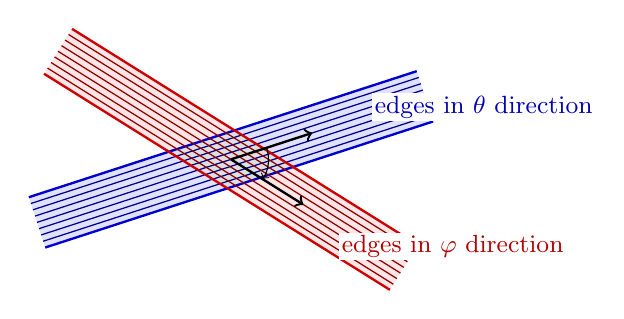
\begin{tikzpicture}[scale=0.7, every node/.style={font=\small}]
        \def\striplen{3.7}
        \def\stripwidth{0.48}

        \begin{scope}[rotate=18]
                \fill[blue!12] (-\striplen,-\stripwidth) rectangle (\striplen,\stripwidth);
        \end{scope}
        \begin{scope}[rotate=-32]
                \fill[red!10] (-\striplen,-\stripwidth) rectangle (\striplen,\stripwidth);
        \end{scope}

        \begin{scope}
                \clip[rotate=18] (-\striplen,-\stripwidth) rectangle (\striplen,\stripwidth);
                \fill[gray!25, rotate=-32] (-\striplen,-\stripwidth) rectangle (\striplen,\stripwidth);
        \end{scope}

        \begin{scope}[rotate=18]
                \foreach \y in {-0.36,-0.24,-0.12,0,0.12,0.24,0.36}
                        \draw[blue!55!black, line width=0.45pt] (-\striplen,\y)--(\striplen,\y);
                \draw[blue!80!black, line width=0.85pt] (-\striplen,-\stripwidth)--(\striplen,-\stripwidth);
                \draw[blue!80!black, line width=0.85pt] (-\striplen,\stripwidth)--(\striplen,\stripwidth);
        \end{scope}
        \begin{scope}[rotate=-32]
                \foreach \y in {-0.36,-0.24,-0.12,0,0.12,0.24,0.36}
                        \draw[red!55!black, line width=0.45pt] (-\striplen,\y)--(\striplen,\y);
                \draw[red!80!black, line width=0.85pt] (-\striplen,-\stripwidth)--(\striplen,-\stripwidth);
                \draw[red!80!black, line width=0.85pt] (-\striplen,\stripwidth)--(\striplen,\stripwidth);
        \end{scope}

        \draw[->, line width=0.85pt] (0,0)--(18:1.55) node[pos=0.94, above, inner sep=1pt] {};
        \draw[->, line width=0.85pt] (0,0)--(-32:1.55) node[pos=0.94, below, inner sep=1pt] {};
        \draw[->] (18:0.68) arc[start angle=18, end angle=-32, radius=0.68];

        \node[blue!70!black, anchor=west, fill=white, inner sep=1pt] at (2.55,0.95) {edges in \(\theta\) direction};
        \node[red!70!black, anchor=west, fill=white, inner sep=1pt] at (1.95,-1.58) {edges in \(\varphi\) direction};
\end{tikzpicture}
\caption{Two streams of edges at a crossing point \(x\).  The two strips overlap in a parallelogram, and the area element of this parallelogram  gives the factor $|\sin(\theta_1 -\theta_2)|$.}
\label{fig:parallelogram}
\end{figure}

The Jacobian change of variables computation, deferred to \Cref{subsec:main-lemmas}, gives the following representation for the crossing functional
\begin{equation}\label{eq:normalized-flux-crossing-representation}
        \operatorname{Cr}(w)=
        \int_{{\mathbb S}^2}\int_0^{2\pi}\int_0^{2\pi}
        g(x,\theta)g(x,\phi)\abs{\sin(\theta-\phi)}
        \,\dd\theta\,\dd\phi\,\sigma(\dd x)\,.
\end{equation}
Pictorially, \Cref{fig:parallelogram} explains why $|\sin(\theta - \phi)|$ shows up in \eqref{eq:normalized-flux-crossing-representation}. Similarly, we get  
\begin{equation}\label{eq:normalized-incidence-identity}
       e(w)= \int_{{\mathbb S}^2}\int_0^{2\pi}a(x,\theta)\,\dd\theta\,\sigma(\dd x)\,.
\end{equation}
We show that one can lower bound $g$ by a function of $a$ pointwise as follows.
\begin{lemma}\label{lem:normalized-bathtub-main}
For almost every \((x,\theta) \in {\mathbb S}^2 \times [0, 2\pi)\), we have 
\begin{equation}\label{eq:normalized-pointwise-bathtub}
    g(x,\theta) \geq \varphi (a (x,\theta))\,,
\end{equation}
where $\varphi : [0,1/(8\pi^2)] \to {\mathbb R}$ is defined by 
\begin{equation}\label{eq:normalized-bathtub-profile}
        \varphi(\alpha):=
        \frac{\sin \tau(\alpha)-\tau(\alpha)\cos \tau(\alpha)}{(4\pi)^2}\,,
\end{equation}
where $\tau(\alpha) \in [0,\pi]$ is determined by $16\pi^2 \alpha =1-\cos  \tau(\alpha).$
\end{lemma}

We will also use that $\alpha \mapsto  \varphi(\alpha)^{2/3}$ is convex on its domain. The proof of \Cref{lem:normalized-bathtub-main} and the convexity calculation are deferred to \Cref{subsec:main-lemmas}. Finally, the most crucial part of the argument will be a version of Busemann's inequality that we will prove in \Cref{sec:busemann}.

\begin{lemma}[Busemann inequality]\label{lem:busemann-circle-main}
For every measurable \(f:[0,2\pi)\to[0,\infty)\),
\begin{equation}\label{eq:busemann-circle-main}
        \int_0^{2\pi}\int_0^{2\pi}
        f(\theta)f(\phi)\abs{\sin(\theta-\phi)}
        \,\dd\theta\,\dd\phi
        \ge
        \frac1{\pi^2}
        \left(\int_0^{2\pi}f(\theta)^{2/3}\,\dd\theta\right)^3.
\end{equation}
\end{lemma}

We now combine all the ingredients above to prove \Cref{thm:continuous-spherical-crossing-main}.



\begin{proof}[Proof of \Cref{thm:continuous-spherical-crossing-main}]
The crossing representation \eqref{eq:normalized-flux-crossing-representation} and Busemann's inequality \eqref{eq:busemann-circle-main} give
\begin{align*}
    \operatorname{Cr}(w)&=\int_{{\mathbb S}^2}\int_0^{2\pi}\int_0^{2\pi}
        g(x,\theta)g(x,\phi)\abs{\sin(\theta-\phi)}
        \,\dd\theta\,\dd\phi\,\sigma(\dd x) \\
        &\geq  \frac1{\pi^2}\int_{{\mathbb S}^2} 
        \left(\int_0^{2\pi}g(x,\theta)^{2/3}\,\dd\theta\right)^3 \sigma(\dd x)\,.
\end{align*}
H\"older's inequality on \(({\mathbb S}^2,\sigma)\) with \(\sigma({\mathbb S}^2)=4\pi\) yields
\begin{align*}
    \operatorname{Cr}(w)&\geq  \frac1{\pi^2}\int_{{\mathbb S}^2} \left(\int_0^{2\pi}g(x,\theta)^{2/3}\,\dd\theta\right)^3 \sigma(\dd x) \geq \frac1{16\pi^4}\left(\int_{{\mathbb S}^2} \int_0^{2\pi}g(x,\theta)^{2/3}\,\dd\theta \,\sigma(\dd x) \right)^3.
\end{align*}
Let $h(\alpha) = \varphi(\alpha)^{2/3}$. Then, the pointwise estimate \Cref{lem:normalized-bathtub-main} gives 
\[
        g(x,\theta)^{2/3}\ge h(a(x,\theta))\,.
\]
By the convexity of \(h\), Jensen's inequality on the space
\({\mathbb S}^2\times[0,2\pi)\) implies
\begin{equation}\label{eq:main-proof-jensen-step}   \int_{{\mathbb S}^2}\int_0^{2\pi}g(x,\theta)^{2/3}\,\dd\theta\,\sigma(\dd x)
        \ge
        8\pi^2\,
        h\left(
        \frac1{8\pi^2}
        \int_{{\mathbb S}^2}\int_0^{2\pi}a(x,\theta)\,\dd\theta\,\sigma(\dd x)
        \right)  =8\pi^2\,h\left(\frac{e(w)}{8\pi^2}\right)\,,
\end{equation}
where the last step uses the identity \eqref{eq:normalized-incidence-identity}.
Let \(t\in[0,\pi]\) be determined by \(\cos t=1-2e(w)\).  The definition of \(\varphi\) gives
\[
        h\left(\frac{e(w)}{8\pi^2}\right)
        =
        \left(\frac{\sin t-t\cos t}{(4\pi)^2}\right)^{2/3}\,.
\]
Substituting this into the preceding bound and using \eqref{eq:main-proof-jensen-step}, we obtain
\[
        \operatorname{Cr}(w)
        \ge
        \frac1{16\pi^4}
        (8\pi^2)^3
        \left(\frac{\sin t-t\cos t}{(4\pi)^2}\right)^2
        =
        \frac{(\sin t-t\cos t)^2}{8\pi^2}\,.
\]
This proves the lower bound. It remains to check sharpness.  For density \(w(x,y)=\II{\{d(x,y)\le t\}}\), we have \(e(w)=(1-\cos t)/2\).  Moreover, we have that
\[
        g(x,\theta)
        =
        \frac1{(4\pi)^2}\int_0^t u\sin u\,\dd u
        =
        \frac{\sin t-t\cos t}{(4\pi)^2}
\]
independently of \((x,\theta)\).  Since $\sigma({\mathbb S}^2)=4\pi$ and 
\[
        \int_0^{2\pi}\int_0^{2\pi}\abs{\sin(\theta-\phi)}\,\dd\theta\,\dd\phi=8\pi\,,
\]
the flux formula \eqref{eq:normalized-flux-crossing-representation} gives
\[
        \operatorname{Cr}(w)
        =32\pi^2
        \left(\frac{\sin t-t\cos t}{(4\pi)^2}\right)^2
        =
        \frac{(\sin t-t\cos t)^2}{8\pi^2}\,.
\]
Hence equality is attained by \(w\).
\end{proof}

\subsection{Proofs of Lemmas}\label{subsec:main-lemmas}
We now give the deferred details for the geometric identities and the one dimensional rearrangement estimate used in the proof of \Cref{thm:continuous-spherical-crossing-main}.  The first two lemmas are change of variables computations for parametrizing a geodesic segment by an interior point, a tangent direction, and the distances to the two endpoint.  The third lemma reduces the pointwise estimate \(g\ge \varphi(a)\) on each geodesic fiber to the bathtub principle.  

\begin{lemma}[Crossing identity]\label{lem:spherical-crossing-jacobian-main}
Let \(w:{\mathbb S}^2\times{\mathbb S}^2\to[0,1]\) be measurable and symmetric, and let \(g\) be defined by \eqref{eq:normalized-g-def}.  Then, we have that
\begin{equation*}
        \operatorname{Cr}(w)=
        \int_{{\mathbb S}^2}\int_0^{2\pi}\int_0^{2\pi}
        g(x,\theta)g(x,\phi)\abs{\sin(\theta-\phi)}
        \,\dd\theta\,\dd\phi\,\sigma(\dd x)\,.
\end{equation*}
\end{lemma}

\begin{proof}
For \(i=1,2\) and $(s_i,r_i)\in\Delta $, set $ y_i^+=\exp_x(s_i v_{x,\theta_i})$ and $y_i^-=\exp_x(-r_i v_{x,\theta_i})$. The map
\[
        (x,\theta_1,\theta_2,s_1,r_1,s_2,r_2)
        \longmapsto (y_1^+,y_1^-,y_2^+,y_2^-)
\]
parametrizes, up to null sets, the ordered endpoint quadruples whose two geodesic segments $[y_1^-y_1^+]$ and $[y_2^-y_2^+]$ cross transversely at \(x\). Here \(\theta_1\) and \(\theta_2\) denote the directions through \(x\) of the geodesic segments \([y_1^-y_1^+]\) and \([y_2^-y_2^+]\), respectively, while \(s_i\) and \(r_i\) represent the signed distances from \(x\) to the corresponding endpoints. It now remains to compute its Jacobian. Work locally in a smooth oriented orthonormal frame and write
\[
        v_i:=v_{x,\theta_i}\,,\qquad n_i:=\partial_{\theta_i}v_{x,\theta_i}\,.
\]
For one segment, if \(\xi\in T_x{\mathbb S}^2\) is the base point change and \(\eta_i\) is the angular change, then the changed endpoint coordinates are
\[
        \cos s_i\,\langle\xi,n_i\rangle+\eta_i\sin s_i\,,
        \qquad
        \cos r_i\,\langle\xi,n_i\rangle-\eta_i\sin r_i\,.
\]
Hence the change determinant for the \(i\)-th segment is
\[
        \abs{\det\begin{pmatrix}
        \cos s_i & \sin s_i\\
        \cos r_i & -\sin r_i
        \end{pmatrix}}
        =\sin(s_i+r_i)\,,
\]
while \(s_i\) and \(r_i\) give the longitudinal directions.  The remaining base point change of coordinates contributes $\abs{\det(n_1,n_2)}=\abs{\sin(\theta_1-\theta_2)}.$ Therefore,
\begin{equation}\label{eq:spherical-crossing-jacobian-main}
        J=
        \sin(s_1+r_1)\sin(s_2+r_2)
        \abs{\sin(\theta_1-\theta_2)}\,.
\end{equation}
Applying this to \eqref{eq:continuous-crossing-functional} and using \(\mu=\sigma/(4\pi)\) gives
\begin{align*}
        \operatorname{Cr}(w)
        &=\frac{1}{(4\pi)^{4}}
        \int_{{\mathbb S}^2}\int_0^{2\pi}\int_0^{2\pi}
        \int_{\Delta}\int_{\Delta}
        w(y_1^+,y_1^-)w(y_2^+,y_2^-) J
        \,\dd r_1\,\dd s_1\,\dd r_2\,\dd s_2
        \,\dd\theta_1\,\dd\theta_2\,\sigma(\dd x) \\
        &=\int_{{\mathbb S}^2}\int_0^{2\pi}\int_0^{2\pi}
        g(x,\theta_1)g(x,\theta_2)
        \abs{\sin(\theta_1-\theta_2)}
        \,\dd\theta_1\,\dd\theta_2\,\sigma(\dd x)\,,
\end{align*}
which proves the claim.
\end{proof}



\begin{lemma}[Edge identity]\label{lem:incidence-identity-main}
Let \(w:{\mathbb S}^2\times{\mathbb S}^2\to[0,1]\) be measurable and symmetric, and let \(a\) be defined by \eqref{eq:normalized-a-def}.  Then, we have that
\[
        e(w)=\int_{{\mathbb S}^2}\int_0^{2\pi}a(x,\theta)\,\dd\theta\,\sigma(\dd x)\,.
\]
\end{lemma}

\begin{proof}
From the proof of \Cref{lem:spherical-crossing-jacobian-main}, the normal Jacobian of the map
\[
        (x,\theta,s,r)\longmapsto
        \left(\exp_x(sv_{x,\theta}),\exp_x(-rv_{x,\theta})\right)
\]
is precisely \(\sin(s+r)\).  For fixed endpoints \((y,z)\), the fiber consists of the points \(x\) on the segment \([yz]\), and its length is \(d(y,z)=s+r\).  This gives
\begin{equation*}\int_{{\mathbb S}^2}\int_0^{2\pi}a(x,\theta)\,\dd\theta\,\sigma(\dd x)=
        \frac1{(4\pi)^2}
        \int_{{\mathbb S}^2}\int_{{\mathbb S}^2}w(y,z)\,\sigma(\dd y)\sigma(\dd z)=e(w)\,.
        \qedhere 
\end{equation*}
\end{proof}
\begin{lemma}\label{lem:spherical-pointwise-inequality}
Let \(w:{\mathbb S}^2\times{\mathbb S}^2\to[0,1]\) be measurable and symmetric, and let \(g\) and $a$ be defined by equations \eqref{eq:normalized-g-def}-\eqref{eq:normalized-a-def} and $\varphi$ be as  \eqref{eq:normalized-bathtub-profile}. Then, for almost every \((x,\theta) \in {\mathbb S}^2 \times [0,2\pi)\), we have
\begin{equation*}
    g(x,\theta)\geq \varphi(a(x,\theta))\,.
\end{equation*}
\end{lemma}

\begin{proof}
Fix \((x,\theta)\). For $(s,r) \in \Delta$  write $q(s,r): =w\left(\exp_x(sv_{x,\theta}),\exp_x(-rv_{x,\theta})\right)$. Let us do a change variables to \(u=s+r\) and \(z=s\).  For \(u \in (0, \pi)\), put
\[
        b(u):=\int_0^u q(z,u-z)\,\dd z\,.
\]
Note that $b(u) \in [0,u]$. Now, equations \eqref{eq:normalized-g-def} and \eqref{eq:normalized-a-def} translate to 
\[
       a(x,\theta)= \frac{1}{ (4\pi)^2}\int_0^\pi \frac{\sin u}{u}b(u)\,\dd u\,,
        \qquad
       g(x,\theta)=\frac{1}{ (4\pi)^2}\int_0^\pi \sin u\,b(u)\,\dd u\,.
\]
Equivalently, let \(\dd\nu(u)=(\sin u/u)b(u)\,\dd u\).  Then \(0\le\dd\nu\le \sin u\,\dd u\), its mass is \((4\pi)^2a(x,\theta)\), and
\[
        g(x,\theta)=\frac{1}{(4\pi)^2}\int_0^\pi u\,\dd\nu(u)\,.
\]
Among all measures dominated by \(\sin u\,\dd u\) with fixed mass, the integral of the increasing cost \(u\) is minimized by filling the interval from the left.  Thus if \(\tau\) is determined by
\[
        (4\pi)^2a(x,\theta)=\int_0^\tau \sin u\,\dd u=1-\cos \tau \,,
\]
then, we have that 
\[
        (4\pi)^2g(x,\theta)
        \ge
        \int_0^\tau  u\sin u\,\dd u
        =\sin \tau -\tau \cos \tau \,.
\]
This is precisely \(g(x,\theta)\ge\varphi(a(x,\theta))\). Moreover, equality occurs when \(\dd\nu=\sin u\,\dd u\) on \([0,\tau ]\) and \(\dd\nu=0\) on \((\tau ,\pi]\), which is equivalent to \(q(s,r)=\II{\{s+r\le \tau \}}\) for almost every \((s,r)\).
\end{proof}

\begin{lemma}\label{lem:normalized-convexity-main}
Let $\varphi$ be defined as in \eqref{eq:normalized-bathtub-profile}.
 Then, the function \(\alpha \mapsto \varphi(\alpha)^{2/3}\) is convex on \([0,1/(8\pi^2)]\).
\end{lemma}

\begin{proof}
First, observe that by chain rule, we have 
\begin{equation*}
    \frac{\dd \varphi}{\dd \tau}(\tau) = \frac{\tau \sin \tau}{(4\pi)^2} \quad \text{ and } \quad \frac{\dd \alpha}{\dd \tau}(\tau) = \frac{\sin \tau}{(4\pi)^2} \; \;\implies \;\; \frac{\dd \varphi }{\dd \alpha}(\alpha) = \tau(\alpha)\,.
\end{equation*}
Let $h(\alpha) = \varphi(\alpha)^{2/3}$. Then, by chain rule again, we get
\[
       h''(\alpha)
        = \frac{2}{9}\,\varphi(\alpha)^{-4/3}\sqb{3\varphi(\alpha)\varphi ''(\alpha)  - \varphi'(\alpha)^2}\,.
\]
Thus, written in terms of $\tau \in (0,\pi)$, the convexity is equivalent to
\[
        3 (1 - \tau \cot \tau ) - \tau^2 \geq 0\,.
\]
Using Euler's partial fraction expansion for $\tau \in (0, \pi)$,
\[
        \cot \tau=\frac1\tau+2\tau\sum_{k=1}^{\infty}\frac1{\tau^2-k^2\pi^2} \implies 1-\tau\cot \tau
        =2\tau^2\sum_{k=1}^{\infty}\frac1{k^2\pi^2-\tau^2}
        \ge
        2\tau^2\sum_{k=1}^{\infty}\frac1{k^2\pi^2}
        =\frac{\tau^2}{3}\,.
\]
Therefore \(h''(\alpha)\ge0\) in the interior of its domain.  Continuity at endpoints gives full convexity.
\end{proof}

\subsection{Planar Theorem}\label{subsec:main-planar}
The same mechanism also gives the Euclidean analogue of \Cref{thm:continuous-spherical-crossing-main}.  Let \(\Omega\subset{\mathbb R}^2\) be compact and convex, let \(A=\operatorname{area}(\Omega)\), and write \(\lambda=A^{-1}\mathcal L^2|_\Omega\) for the normalized Lebesgue measure, or uniform measure.  For a measurable symmetric \(w:\Omega\times\Omega\to[0,1]\), set
\[
        e_\Omega(w)=\int_{\Omega}\int_{\Omega}w(y,z)\,\lambda(\dd y)\lambda(\dd z)\,,
\]
and let \(\operatorname{Cr}_\Omega(w)\) be the straight-line crossing functional on \(\Omega\), defined analogously to \eqref{eq:continuous-crossing-functional}.

\begin{theorem}\label{thm:continuous-planar-crossing-main}
For every compact convex \(\Omega\subset{\mathbb R}^2\) with nonempty interior and every measurable symmetric \(w:\Omega\times\Omega\to[0,1]\), we have
\begin{equation}\label{eq:continuous-planar-crossing-main}
        \operatorname{Cr}_\Omega(w)
        \ge
        \frac{8}{9\pi^2}\,e_\Omega(w)^3\,.
\end{equation}
\end{theorem}

\begin{proof}
Let us extend $w$ to ${\mathbb R}^2 \times {\mathbb R}^2$ by $0$. For \(\theta\in[0,2\pi)\), write \(v_\theta=(\cos\theta,\sin\theta)\) and define
\begin{align*}
        g_\Omega(x,\theta)
        &:=\frac{1}{A^2}\int_{0}^\infty\int_{0}^\infty
        (s+r)w(x+sv_\theta,x-rv_\theta)\,\dd r\dd s\,,\\
        a_\Omega(x,\theta)
        &:=\frac{1}{A^2}\int_{0}^\infty\int_{0}^\infty
        w(x+sv_\theta,x-rv_\theta)\,\dd r\dd s\,.
\end{align*}
By the analogous computation to \Cref{lem:incidence-identity-main} and \Cref{lem:spherical-crossing-jacobian-main}, the Euclidean crossing  Jacobian is given by
\((s+r)(s'+r')\abs{\sin(\theta-\phi)}\), so we can write 
\[
\begin{aligned}
        \operatorname{Cr}_\Omega(w)
        &=\int_\Omega\int_0^{2\pi}\int_0^{2\pi}
        g_\Omega(x,\theta)g_\Omega(x,\phi)\abs{\sin(\theta-\phi)}
        \,\dd\theta \, \dd\phi \, \dd x\,,\\
        e_\Omega(w)
        &=\int_\Omega\int_0^{2\pi}a_\Omega(x,\theta)\,\dd\theta \, \dd x\,.
\end{aligned}
\]
As in the spherical proof, Busemann's inequality and H\"older give
\begin{equation}\label{eq:planar-holder-step-main}
        \operatorname{Cr}_\Omega(w)
        \ge
        \frac1{\pi^2A^2}
        \left(\int_\Omega\int_0^{2\pi}g_\Omega(x,\theta)^{2/3}\,\dd\theta \, \dd x\right)^3\,.
\end{equation}
For fixed \((x,\theta)\), analogously to \Cref{lem:spherical-pointwise-inequality} we can prove that 
\begin{equation*}
    g_\Omega(x,\theta) \geq \frac{2\sqrt{2} }{3} A  \, a_\Omega(x,\theta)^{3/2} \implies  \int_\Omega\int_0^{2\pi}g_\Omega(x,\theta)^{2/3}\,\dd\theta\, \dd x
        \ge
        \left(\frac{2\sqrt2}{3} A\right)^{2/3}e_\Omega(w)\,.
\end{equation*}
Substitution into \eqref{eq:planar-holder-step-main} yields
\[
        \operatorname{Cr}_\Omega(w)
        \ge
        \frac1{\pi^2A^2}
        \left(\frac{2\sqrt2}{3} A\right)^2e_\Omega(w)^3
        =
        \frac8{9\pi^2} e_\Omega(w)^3\,. \qedhere \]
\end{proof}
One can think of \Cref{thm:continuous-planar-crossing-main} as a local version of \Cref{thm:continuous-spherical-crossing-main}. Indeed, after transferring a planar drawing to a sufficiently small local chart on the sphere, the planar lemmas used in the proof of \Cref{thm:continuous-planar-crossing-main} become immediate corollaries of the corresponding lemmas in the spherical setting. Moreover, if the plane can be tiled by copies of $\Omega$, then \Cref{thm:continuous-planar-crossing-main} can be deduced directly from \Cref{thm:continuous-spherical-crossing-main}: one covers the sphere with rescaled copies of the planar drawing, with the scales tending to zero, so that the resulting error tends to zero as well. 

\section{Busemann's Inequality}\label{sec:busemann}

In this section, we prove Busemann’s inequality~\ref{lem:busemann-circle-main}. If one interprets $f^{1/3}$ as the radial function of a star-shaped body in the plane, then the inequality has a geometric meaning. It states that the expected area of the triangle formed by the center and two uniformly randomly sampled points from the body is minimized when the body is an ellipsoid. This statement for convex bodies is originally proved in \cite{Busemann53}. We give an alternative proof tailored to our purposes.  We start by proving a linear version of the inequality, and then we lift it up.

\begin{lemma}\label{lem:busemann-line}
For every measurable function $q:{\mathbb R}\to[0,\infty)$,
\begin{equation}\label{eq:busemann-line}
        \int_{{\mathbb R}}\int_{{\mathbb R}}q(u)q(v)\abs{u-v}\,\dd u\dd v
        \ge
        \frac{2}{\pi^2}
        \left(\int_{{\mathbb R}}q(u)^{2/3}\,\dd u\right)^3\,.
\end{equation}
\end{lemma}

\begin{proof}
By truncating $q$ to $q_n(u):=(q(u) \wedge n)\II{\{\abs{u}\le n\}}$ and using monotone convergence on both sides, it is enough to prove the estimate for bounded $q$ supported on a finite interval.  On such an interval we may approximate in $L^1$ by functions which are positive and continuous on their support; since the kernel $\abs{u-v}$ is bounded on a fixed compact set and since $|a^{2/3}-b^{2/3}|\le |{a-b}|^{2/3}$, the estimate passes to the limit.  Thus, without loss of generality, we assume that $q$ is positive and continuous on its support $[a,b]$, and that it integrates to $1$. Define
\[
        Q(x):=\int_a^x q(u)\,\dd u\,.
\]
Now we note that equality $|u - v| = \int_{{\mathbb R}}\II{\{u<x<v\}}+\II{\{v<x<u\}}\,\dd x$ lets us rewrite the left hand side as
\begin{equation}\label{eq:busemann-line-layercake}
\begin{aligned}
        \int_{{\mathbb R}}\int_{{\mathbb R}}q(u)q(v)\abs{u-v}\,\dd u\dd v
        &=2\int_a^b Q(x)(1-Q(x))\,\dd x\,.
\end{aligned}
\end{equation}
Define $x(t)$ by $Q(x(t))=t$ for $t\in(0,1)$.  Then $x'(t)=q(x(t))^{-1}$, so the equality \eqref{eq:busemann-line-layercake} becomes
\begin{equation}\label{eq:busemann-line-quantile-energy}
        \int_{{\mathbb R}}\int_{{\mathbb R}}q(u)q(v)\abs{u-v}\,\dd u\dd v
        =2 \int_0^1 t(1-t) q(x(t))^{-1}\,\dd t = 2\int_0^1 t(1-t) \, y(t)^3\,\dd t\,,
\end{equation}
where $y(t):=q(x(t))^{-1/3}$. Similarly, by the change of variables $u = x(t)$, we get 
\begin{equation}\label{eq:busemann-line-quantile-mass}
        \int_{{\mathbb R}}q(u)^{2/3}\,\dd u
        =\int_0^1 q(x(t))^{-1/3}\,\dd t = \int_0^1 y(t)\,\dd t\,.
\end{equation}
Now, H\"older's inequality gives
\[
        \Biggl({\int_0^1 y(t)\,\dd t\Biggr)}^3
        \le
        \Biggl(\int_0^1 t(1-t) \, y(t)^3\,\dd t\Biggr)
        \Biggl(\int_0^1 \frac{\dd t}{\sqrt{t(1-t)}}\Biggr)^{2} = \pi^2 \int_0^1 t(1-t) \, y(t)^3\,\dd t\,.
\]
Hence, we are done.
\end{proof}

\begin{proof}[Proof of \Cref{lem:busemann-circle-main}]
Let us define a bilinear form $B$ by
\[
        B(f,h):=\int_0^{2\pi}\int_0^{2\pi}
        f(\theta)h(\phi)\abs{\sin(\theta-\phi)}\,\dd\theta\dd\phi \,.
\]
First replace $f$ by the average $\bar f(\theta) := [f(\theta)+f(\theta+\pi)]/2,$ where angles are taken modulo $2\pi$.  The kernel $\abs{\sin(\theta-\phi)}$ is unchanged when either variable is shifted by $\pi$, so bilinearity gives $B(\bar f,\bar f)=B(f,f)$.  Since $x\mapsto x^{2/3}$ is concave, we have
\[
        \int_0^{2\pi} \bar f(\theta)^{2/3}\,\dd\theta
        \ge
        \int_0^{2\pi} f(\theta)^{2/3}\,\dd\theta\,.
\]
We can therefore assume without loss of generality that $f$ is $\pi$-periodic. Up to a null set of directions, write $u=\tan\theta$ with $\theta\in(-\pi/2,\pi/2)$, and define
\[
        q(u):=\frac{f(\tan^{-1} u)}{\,\,(1+u^2)^{3/2}}\,.
\]
If $u = \tan \theta$ and $v = \tan \phi$, we note that 
\[
        \abs{\sin(\theta-\phi)}
        =\frac{\abs{u-v}}{\sqrt{(1+u^2)(1+v^2)}}
        \quad \text{ and } \quad 
         \frac{\dd\theta}{\dd u}=\frac{1}{1+u^2}\,.
\]
Hence, this change of variables gives 
\begin{equation}\label{eq:busemann-circle-to-line-energy}
        B(f,f)
        =4\int_{-\pi/2}^{\pi/2}\int_{-\pi/2}^{\pi/2}
        f(\theta)f(\phi)\abs{\sin(\theta-\phi)}\,\dd\theta\dd\phi
        =4\int_{{\mathbb R}}\int_{{\mathbb R}}q(u)q(v)\abs{u-v}\,\dd u\dd v\,.
\end{equation}
Also, with the same change of variables,
\begin{equation}\label{eq:busemann-circle-to-line-mass}
        \int_0^{2\pi}f(\theta)^{2/3}\,\dd\theta
        =2\int_{{\mathbb R}}q(u)^{2/3}\,\dd u\,.
\end{equation}
Applying \Cref{lem:busemann-line} to $q$ and using \eqref{eq:busemann-circle-to-line-energy} and \eqref{eq:busemann-circle-to-line-mass}, we obtain
\[
        B(f,f)
        \ge
        4\cdot\frac{2}{\pi^2}
        \left(\int_{{\mathbb R}}q(u)^{2/3}\,\dd u\right)^3
        =
        \frac1{\pi^2}
        \left(\int_0^{2\pi}f(\theta)^{2/3}\,\dd\theta\right)^3\,.
\]
This is exactly \eqref{eq:busemann-circle-main}.
\end{proof}

\begin{remark}
The  H\"older equality case in the proof of \Cref{lem:busemann-line} holds when  $y(t)=q(x(t))^{-1/3}$ is proportional to $1/\sqrt{t(1-t)}$.  In the proof of \Cref{lem:busemann-circle-main}, this gives densities coming from centered ellipses.
\end{remark}

\section{Reduction}\label{sec:reduction}
In this section, we reduce the discrete theorems to the continuous ones. Since the arguments for the spherical and planar cases are very similar, we only carry out the reduction of \Cref{thm:main-spherical} to \Cref{thm:continuous-spherical-crossing-main}.  The idea is to replace each vertex by a small smooth cloud of radius \(\delta\), and replace each edge by the product of its two endpoint clouds.  For fixed \(\delta\), the smoothed vertex density is uniformly close to \(1\) once \(n\) gets large.  The main point is to show that this smoothing does not create many new crossings. 

We first prove a lemma showing that if a perturbation of a pair of non-crossing edges causes them to cross, then at least one endpoint must be close to the other edge. For illustration, see \Cref{fig:perturbation}.

\begin{lemma} \label{lem:reduction-new-crossing-geometric}
There are absolute positive constants \(C\) and \(c\) such that the following property holds.  Suppose \(0<\alpha<1/10\), let \(0<\delta\le c\alpha^2\), and let $x_1,x_2,x_3,x_4 \in {\mathbb S}^2$ be four points satisfying
\[
        \alpha\le d(x_1,x_2),d(x_3,x_4)\le \pi-\alpha\,.
\]
Assume that \([x_1x_2]\) and \([x_3x_4]\) do not cross.  Suppose \(y_1,y_2,y_3,y_4\in{\mathbb S}^2\) are such that $d(x_i, y_i) \leq \delta$ and the perturbed segments \([y_1y_2]\) and \([y_3y_4]\) cross, then
\begin{equation}\label{eq:reduction-new-crossing-nearby-endpoint}
        \min\{d(x_1,[x_3x_4]),d(x_2,[x_3x_4]),
              d(x_3,[x_1x_2]),d(x_4,[x_1x_2])\}
        \le C{\delta}/{\alpha}\,.
\end{equation}
\end{lemma}


\begin{figure}[t]
    \centering
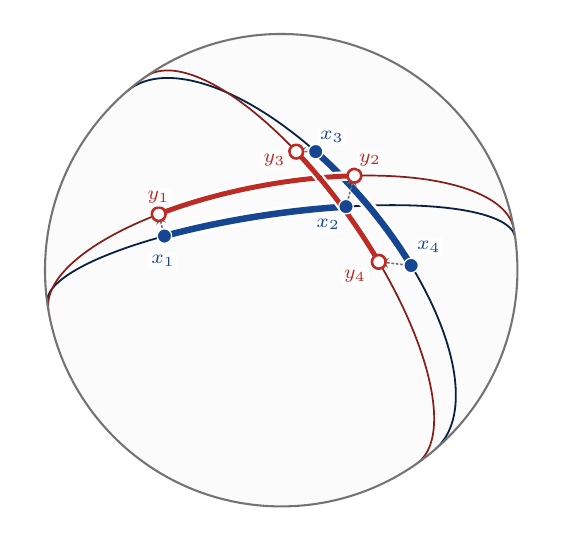
\begin{tikzpicture}[
    x=1cm,y=1cm,
    line cap=round,
    line join=round,
    font=\scriptsize,
    spheregrid/.style={draw=black!24, line width=0.45pt},
    xsupport/.style={draw=rmccOriginalBlue!45!black, line width=0.65pt},
    ysupport/.style={draw=rmccPerturbRed!70!black, line width=0.62pt},
    origedge/.style={draw=rmccOriginalBlue, line width=2.35pt,
        preaction={draw=white, line width=4.6pt}},
    pertedge/.style={draw=rmccPerturbRed, line width=1.80pt,
        preaction={draw=white, line width=3.5pt}},
    moveline/.style={draw=black!55, densely dotted, line width=0.60pt, -stealth},
    xpoint/.style={circle, fill=rmccOriginalBlue, draw=white, line width=0.45pt, inner sep=1.85pt},
    ypoint/.style={circle, fill=white, draw=rmccPerturbRed, line width=0.95pt, inner sep=1.75pt},
    labelbox/.style={fill=white, fill opacity=0.88, text opacity=1, inner sep=1.1pt, rounded corners=0.7pt}
]

\definecolor{rmccOriginalBlue}{RGB}{22,70,145}
\definecolor{rmccPerturbRed}{RGB}{190,42,36}

\path[use as bounding box] (-3.22,-3.08) rectangle (3.22,3.08);
\def\R{3.00}

\pgfmathsetmacro{\Ga}{3.00}
\pgfmathsetmacro{\Gb}{0.72}
\pgfmathsetmacro{\Grot}{8}
\pgfmathsetmacro{\Ha}{3.00}
\pgfmathsetmacro{\Hb}{1.372}
\pgfmathsetmacro{\Hrot}{-49.21}

\pgfmathsetmacro{\Ua}{3.00}
\pgfmathsetmacro{\Ub}{1.10}
\pgfmathsetmacro{\Urot}{10}
\pgfmathsetmacro{\Va}{3.00}
\pgfmathsetmacro{\Vb}{1.10}
\pgfmathsetmacro{\Vrot}{-55}

\coordinate (x1) at ({\Ga*cos(118)*cos(\Grot)-\Gb*sin(118)*sin(\Grot)},
                     {\Ga*cos(118)*sin(\Grot)+\Gb*sin(118)*cos(\Grot)});
\coordinate (x2) at ({\Ga*cos(72)*cos(\Grot)-\Gb*sin(72)*sin(\Grot)},
                     {\Ga*cos(72)*sin(\Grot)+\Gb*sin(72)*cos(\Grot)});
\coordinate (x3) at ({\Ha*cos(106.54)*cos(\Hrot)-\Hb*sin(106.54)*sin(\Hrot)},
                     {\Ha*cos(106.54)*sin(\Hrot)+\Hb*sin(106.54)*cos(\Hrot)});
\coordinate (x4) at ({\Ha*cos(69.87)*cos(\Hrot)-\Hb*sin(69.87)*sin(\Hrot)},
                     {\Ha*cos(69.87)*sin(\Hrot)+\Hb*sin(69.87)*cos(\Hrot)});

\coordinate (y1) at ({\Ua*cos(118)*cos(\Urot)-\Ub*sin(118)*sin(\Urot)},
                     {\Ua*cos(118)*sin(\Urot)+\Ub*sin(118)*cos(\Urot)});
\coordinate (y2) at ({\Ua*cos(68)*cos(\Urot)-\Ub*sin(68)*sin(\Urot)},
                     {\Ua*cos(68)*sin(\Urot)+\Ub*sin(68)*cos(\Urot)});
\coordinate (y3) at ({\Va*cos(112)*cos(\Vrot)-\Vb*sin(112)*sin(\Vrot)},
                     {\Va*cos(112)*sin(\Vrot)+\Vb*sin(112)*cos(\Vrot)});
\coordinate (y4) at ({\Va*cos(78)*cos(\Vrot)-\Vb*sin(78)*sin(\Vrot)},
                     {\Va*cos(78)*sin(\Vrot)+\Vb*sin(78)*cos(\Vrot)});
\coordinate (q)  at ({\Ua*cos(76.85)*cos(\Urot)-\Ub*sin(76.85)*sin(\Urot)},
                     {\Ua*cos(76.85)*sin(\Urot)+\Ub*sin(76.85)*cos(\Urot)});

\fill[black!1.5] (0,0) circle (\R);
\begin{scope}
    \clip (0,0) circle (\R);

    \draw[xsupport] plot[variable=\t, domain=0:180, samples=100]
        ({\Ga*cos(\t)*cos(\Grot)-\Gb*sin(\t)*sin(\Grot)},
         {\Ga*cos(\t)*sin(\Grot)+\Gb*sin(\t)*cos(\Grot)});
    \draw[xsupport] plot[variable=\t, domain=0:180, samples=100]
        ({\Ha*cos(\t)*cos(\Hrot)-\Hb*sin(\t)*sin(\Hrot)},
         {\Ha*cos(\t)*sin(\Hrot)+\Hb*sin(\t)*cos(\Hrot)});

    \draw[ysupport] plot[variable=\t, domain=0:180, samples=100]
        ({\Ua*cos(\t)*cos(\Urot)-\Ub*sin(\t)*sin(\Urot)},
         {\Ua*cos(\t)*sin(\Urot)+\Ub*sin(\t)*cos(\Urot)});
    \draw[ysupport] plot[variable=\t, domain=0:180, samples=100]
        ({\Va*cos(\t)*cos(\Vrot)-\Vb*sin(\t)*sin(\Vrot)},
         {\Va*cos(\t)*sin(\Vrot)+\Vb*sin(\t)*cos(\Vrot)});
\end{scope}
\draw[black!55, line width=0.75pt] (0,0) circle (\R);

\draw[origedge] plot[variable=\t, domain=118:72, samples=90]
    ({\Ga*cos(\t)*cos(\Grot)-\Gb*sin(\t)*sin(\Grot)},
     {\Ga*cos(\t)*sin(\Grot)+\Gb*sin(\t)*cos(\Grot)});
\draw[origedge] plot[variable=\t, domain=106.54:69.87, samples=80]
    ({\Ha*cos(\t)*cos(\Hrot)-\Hb*sin(\t)*sin(\Hrot)},
     {\Ha*cos(\t)*sin(\Hrot)+\Hb*sin(\t)*cos(\Hrot)});

\draw[moveline] (x1) -- (y1);
\draw[moveline] (x2) -- (y2);
\draw[moveline] (x3) -- (y3);
\draw[moveline] (x4) -- (y4);

\draw[pertedge] plot[variable=\t, domain=118:68, samples=90]
    ({\Ua*cos(\t)*cos(\Urot)-\Ub*sin(\t)*sin(\Urot)},
     {\Ua*cos(\t)*sin(\Urot)+\Ub*sin(\t)*cos(\Urot)});
\draw[pertedge] plot[variable=\t, domain=112:78, samples=70]
    ({\Va*cos(\t)*cos(\Vrot)-\Vb*sin(\t)*sin(\Vrot)},
     {\Va*cos(\t)*sin(\Vrot)+\Vb*sin(\t)*cos(\Vrot)});

\node[xpoint] at (x1) {};
\node[xpoint] at (x2) {};
\node[xpoint] at (x3) {};
\node[xpoint] at (x4) {};
\node[ypoint] at (y1) {};
\node[ypoint] at (y2) {};
\node[ypoint] at (y3) {};
\node[ypoint] at (y4) {};
\fill[rmccPerturbRed] (q) circle (1.05pt);

\node[labelbox, text=rmccOriginalBlue, anchor=south] at (-1.50, 0) {$x_1$};
\node[labelbox, text=rmccOriginalBlue, anchor=north east] at ( 0.79, 0.70) {$x_2$};
\node[labelbox, text=rmccOriginalBlue, anchor=south west] at ( 0.45, 1.58) {$x_3$};
\node[labelbox, text=rmccOriginalBlue, anchor=west] at ( 1.68, 0.3) {$x_4$};

\node[labelbox, text=rmccPerturbRed, anchor=south] at (-1.56, 0.80) {$y_1$};
\node[labelbox, text=rmccPerturbRed, anchor=south west] at ( 0.94, 1.28) {$y_2$};
\node[labelbox, text=rmccPerturbRed, anchor=east] at ( 0.1, 1.4) {$y_3$};
\node[labelbox, text=rmccPerturbRed, anchor=south west] at ( 0.75, -0.2) {$y_4$};

\end{tikzpicture}
    \caption{Curves $[x_1x_2]$ and $[x_3x_4]$ are non-crossing, but they begin to cross after a small perturbation. Observe that the endpoint $x_2$ is close to the edge $[x_3x_4]$.}
    \label{fig:perturbation}
\end{figure}


\begin{proof}
In the following argument, the absolute constants $c$ and $C$ may vary from line to line. We denote the Hausdorff distance by $d_H$. Recall that the Hausdorff distance between two closed sets is the greatest distance from a point in one set to the nearest point in the other.

We first record the only geometric estimate we need. If \(d(x,x')\in[\alpha,\pi-\alpha]\), and  $y,y' \in {\mathbb S}^2$ satisfy \(d(x,y),d(x',y')\le\delta\) then
\begin{equation}\label{eq:reduction-segment-hausdorff}
        d_H([xx'],[yy'])\le C{\delta}/{\alpha}\,.
\end{equation}
To see this, compare the supporting great circles.  If
\(n=(x\times x')/\abs{x\times x'}\) and \(n'=(y\times y')/\abs{y\times y'}\) are unit normals, then \(\abs{x\times x'}=\sin d(x,x')\ge\sin\alpha\geq c\alpha\). On the other hand, by linearity, the cross product changes by at most \(O(\delta)\).  Thus, after choosing the sign of \(n'\),
\[
        \abs{n-n'}\le C{\delta}/{\alpha}\,.
\]
So the supporting great circles \(\Gamma(xx')\) and \(\Gamma(yy')\) are within Hausdorff distance \(O(\delta/\alpha)\).  Rotating \(\Gamma(xx')\) onto \(\Gamma(yy')\) moves every point by \(O(\delta/\alpha)\), and sends the endpoints \(x,x'\) to points within \(O(\delta/\alpha)\) of \(y,y'\).  On a fixed circle, shorter arcs whose endpoints are within \(O(\delta/\alpha)\) have Hausdorff distance \(O(\delta/\alpha)\), since their lengths remain at most \(\pi-\alpha/2\).  This proves \eqref{eq:reduction-segment-hausdorff}.

Now, join each \(x_i\) to \(y_i\) by the short geodesic path and move the four endpoints continuously.  Since both original edge lengths lie in \([\alpha,\pi-\alpha]\), all intermediate edge lengths remain bounded away from \(0\) and \(\pi\), if \(c\) is chosen sufficiently small.  At time \(0\) the two closed segments are disjoint, while at time \(1\) they cross.  Let \(t\) be the first time at which the two closed moving segments meet.  The first meeting cannot be a transverse interior-interior crossing, since such a crossing would persist for earlier time.  Hence, at time \(t\), an endpoint of one moving segment lies on the other moving segment. Suppose at time $t$, edges are $[z_1z_2]$ and $[z_3z_4]$. Without loss of generality, suppose $z_1 \in [z_3z_4]$. Then,
\[
        d(x_1,[x_3x_4])
        \le d(x_1,z_1)
             +d_H([z_3z_4],[x_3x_4])
        \le \delta+C{\delta}/{\alpha}
        \le C{\delta}/{\alpha}\,.
\]
This concludes the proof.
\end{proof}

Next, we bound the number of edge–vertex pairs for which the vertex lies close to the edge. This bound will later be used to show that only a small number of new crossings are created. For \(A\subset {\mathbb S}^2\), write
\[
        N_r(A):=\{x\in{\mathbb S}^2:d(x,A)<r\}\,.
\]
\begin{lemma}\label{lem:reduction-uniform-counts}
Let \(P_n=\{p_n(v):v\in V(G_n)\}\), and assume \(n^{-1}\sum_{p\in P_n}\delta_p\Rightarrow\mu\).  Then, for any fixed radius \(r\in(0,\pi/2)\),
\begin{equation}\label{eq:reduction-uniform-cap-count}
        \sup_{z\in{\mathbb S}^2}
        \frac1n\#\{p\in P_n: p \in N_r(z)\}
        \le
        \frac{1-\cos r}{2}+o_r(1)\,,
\end{equation}
\begin{equation}\label{eq:reduction-uniform-tube-count}
        \sup_{\Gamma}
        \frac1n\#\{p\in P_n:p\in N_r(\Gamma)\}
        \le
        \sin r+o_r(1)\,,
\end{equation}
where the second supremum is over all great circles \(\Gamma\subset{\mathbb S}^2\).  Here \(o_r(1)\to0\) as \(n\to\infty\) with \(r\) fixed.
\end{lemma}

\begin{proof}
We prove the tube estimate; the proof for caps is identical.  Suppose the estimate fails for some fixed \(r\).  Then there is a subsequence, still denoted by \(n\), and great circles \(\Gamma_n\) such that
\[
        \frac1n\#(P_n\cap N_r(\Gamma_n))
        \ge \sin r+\varepsilon
\]
for some \(\varepsilon>0\).  The space of great circles is compact, so after passing to a further subsequence we may assume \(\Gamma_n\to\Gamma\).  For every \(\gamma>0\), and all large \(n\), we have $ N_r(\Gamma_n)\subset \overline{N_{r+\gamma}(\Gamma)}$. By weak convergence,
\[
        \limsup_{n\to\infty}\frac1n\#(P_n\cap N_r(\Gamma_n))
        \le
        \mu\bigl(\overline{N_{r+\gamma}(\Gamma)}\bigr)
        =\sin(r+\gamma)\,.
\]
Letting \(\gamma\downarrow0\) gives a contradiction.  The cap estimate follows from  $\mu(N_r(x)) = (1-\cos r)/2$ and analogous argument.
\end{proof}

We can finally carry out the precise reduction, using the ingredients above.
\begin{proposition}[Reduction]\label{prop:discrete-continuous-reduction}
Let \({\mathcal D}_n=(G_n,p_n)\) be a good uniform sequence of spherical geodesic drawings. There are positive constants $c$ and $C$, such that for every fixed \(\delta \in (0,c)\), there are smooth functions $\rho_{n,\delta}:{\mathbb S}^2\to[0,\infty)$ and $ w_{n,\delta}:{\mathbb S}^2\times{\mathbb S}^2\to[0,\infty)$ with the following properties.
\begin{itemize}
    \item[(i)]  $\rho_{n, \delta}$ is a probability density on ${\mathbb S}^2$ that uniformly converges to the uniform density $1$.  
    \begin{equation}\label{eq:reduction-rho-close}
         \int_{{\mathbb S}^2}\rho_{n,\delta}(x)\,\mu(\dd x)=1
        \quad \text{ and } \quad 
        \norm{\rho_{n,\delta}-1}_{L^\infty(\mu)}\to0\,.
    \end{equation}
    \item[(ii)] The edge density $w_{n,\delta}$ is symmetric, $w_{n,\delta}(x,y)\leq \rho_{n,\delta}(x)\rho_{n,\delta}(y)$, and 
    \begin{equation}
        e(w_{n,\delta}) = 2|E(G_n)|/n^2\,.
    \end{equation}
    \item[(iii)] For fixed $\delta$ and growing $n\to \infty$, the crossing density is bounded: 
    \begin{equation}\label{eq:reduction-crossing-bound}
    \operatorname{Cr}(w_{n,\delta}) \leq 
        8\,\frac{\operatorname{cr}({\mathcal D}_n)}{n^4}
        +C\sqrt{\delta}+o_\delta(1)\,.
\end{equation}
\end{itemize}
\end{proposition}

\begin{proof}
Fix $\delta \in (0,c)$.  Choose a smooth nonnegative radial kernel $K:{\mathbb S}^2\times{\mathbb S}^2\to[0,\infty)$ such that \(K(x,y)\) depends only on \(d(x,y)\), is supported on \(d(x,y)<\delta\), and is normalized so that
\[
        \int_{{\mathbb S}^2}K(x,y)\,\mu(\dd x)=1
        \qquad\text{for every }y\in{\mathbb S}^2\,.
\]
For each vertex \(v\in V(G_n)\), let us identify $v$ with $p_n(v) \in {\mathbb S}^2$. Write  \(K_v(x)=K(x,v)\) and define
\begin{equation}\label{eq:reduction-rho-definition-simple}
        \rho_{n,\delta}(x)=\frac1n\sum_{v\in V(G_n)}K_v(x)=\int_{{\mathbb S}^2}K(x,y)\,\nu_n(\dd y),
        \quad \text{ where }
        \nu_n=\frac1n\sum_{v\in V(G_n)}\delta_{v}\,.
\end{equation}
This shows that \(\rho_{n,\delta}\) is a probability density.  Since \(\nu_n\Rightarrow\mu\) and the family
\(\{K(x,\cdot):x\in{\mathbb S}^2\}\) is compact in \(C({\mathbb S}^2)\), the convergence of these integrals is uniform in \(x \in {\mathbb S}^2\).  Hence
\[
        \rho_{n,\delta}(x)\to
        \int_{{\mathbb S}^2}K(x,y)\,\mu(\dd y)=1
        \qquad\text{uniformly in }x\,,
\]
which proves \eqref{eq:reduction-rho-close}. Let \(\vec E(G_n)\) denote the set of the two orientations of each edge of \(G_n\), and define
\begin{equation}\label{eq:reduction-w-definition-simple}
         w_{n,\delta}(x,y)
        =
        \frac1{n^2}\sum_{(u,v)\in\vec E(G_n)}K_u(x)K_v(y)\,.
\end{equation}
This function is symmetric.  Moreover, from here we see $  w_{n,\delta}(x,y) \leq \rho_{n,\delta}(x)\rho_{n,\delta}(y)$. Also, integrating above, we obtain $e(w_{n,\delta}) = 2|E(G_n)|/n^2$. It now remains to compare crossings. Expanding \(w_{n, \delta }\), we observe that
\begin{equation}\label{eq:reduction-crossing-expanded-simple}
            \operatorname{Cr}(w_{n,\delta})
        =\frac1{n^4}
        \sum_{\substack{(a,b)\in\vec E(G_n) \\ (u,v)\in\vec E(G_n)}}
        \Pr\bigl([U_uU_v]\text{ crosses }[U_aU_b]\bigr)\,,
\end{equation}
where, for each occurrence of a vertex \(v\), the random point \(U_v\) is sampled independently from the density \(K_v\,\mu\).  Thus every sampled endpoint lies within spherical distance \(\delta\) of the original endpoint. We decompose the ordered pairs in \eqref{eq:reduction-crossing-expanded-simple}.  Ordered pairs of oriented edges sharing a vertex clearly contribute only \(O(1/n)\).   If two independent edges cross in the original drawing, their unordered pair contributes at most eight ordered and oriented terms to \eqref{eq:reduction-crossing-expanded-simple}.  Hence all originally crossing independent pairs contribute at most
\[
        8\,\frac{\operatorname{cr}({\mathcal D}_n)}{n^4}.
\]
It remains to control independent pairs of edges that do not cross in the original drawing but may cross after the endpoint perturbations.

Call an unordered independent non-crossing pair of edges \(\{x_1x_2,\,x_3x_4\}\) dangerous if there exist points $y_i \in {\mathbb S}^2$ with $d(x_i, y_i) \leq \delta$ such that  \([y_1y_2]\) crosses \([y_3y_4]\).  It suffices to show that the number of dangerous pairs of edges  is at most $[C\sqrt{\delta} +o_\delta(1)]n^4$. 

Let \(c_0,C_0\) be the constants from \Cref{lem:reduction-new-crossing-geometric}.  Choose a large constant \(A\ge 1/\sqrt{c_0}\), and set $\alpha=A\sqrt{\delta}.$ If \(c\) is small enough, we may assume \(0<\alpha<1/10\).  Then \(\delta\le c_0\alpha^2\), so \Cref{lem:reduction-new-crossing-geometric} applies to every pair of edges whose lengths both lie in \([\alpha,\pi-\alpha]\).

First discard the unstable edges, namely those with length outside \([\alpha,\pi-\alpha]\).  For each endpoint $p$, the other endpoint of such an edge must lie in the \(\alpha\)-cap around \(p\) or in the \(\alpha\)-cap around \(-p\).  By \Cref{lem:reduction-uniform-counts} \eqref{eq:reduction-uniform-cap-count}, the number of unstable edges is at most $C[\alpha^2+o_\alpha(1)]n^2$. Hence, the number of edge pairs containing at least one unstable edge is at most $C[\alpha^2+o_\alpha(1)]n^4.$

Consider now a dangerous pair \(\{x_1x_2, \, x_3x_4\}\) in which both edges are stable.  By \Cref{lem:reduction-new-crossing-geometric}, one endpoint of one edge is within $R = C_0 \delta / \alpha$ of the other edge segment.  By decreasing \(c\) again, assume \(R<\pi/2\).  Fix a stable edge \(x_1x_2\).  If \(\Gamma({x_1x_2})\) is its supporting great circle, then
\[
        N_R([x_1x_2])\subseteq N_R(\Gamma({x_1x_2}))\,.
\]
Thus \Cref{lem:reduction-uniform-counts} gives, uniformly in \(x_1x_2\),
\[
        \#\{v\in V(G_n):v\in N_R([x_1x_2])\}
        \le
        \bigl(\sin R+o_R(1)\bigr)n
        \le
        \bigl(CR+o_R(1)\bigr)n\,.
\]
After choosing this near endpoint of the second edge, there are at most \(n\) choices for its other endpoint.  Summing over the at most \(n^2\) choices of the base edge gives at most $[CR + o_R(1)]n^4$ stable dangerous pairs. Combining the bounds above and using \(\alpha=O(\sqrt{\delta})\) and \(R=O(\sqrt{\delta})\), we get that the number of dangerous pairs is at most
\[        \bigl(C\alpha^2+CR+o_\delta(1)\bigr)n^4
        \le
        \bigl(C\sqrt{\delta}+o_\delta(1)\bigr)n^4\,.
\]
This concludes the proof.
\end{proof}

We also mention an easy corollary of \Cref{thm:continuous-spherical-crossing-main}.

\begin{corollary}\label{cor:near-uniform}
Let \(\rho\) be a probability density on \({\mathbb S}^2\) with $\norm{\rho-1}_{L^\infty(\mu)}\le\eta$. Let \(w:{\mathbb S}^2\times{\mathbb S}^2\to[0,\infty)\) be a symmetric function such that $w(x,y)\leq \rho(x)\rho(y)$. If $t \in [0,\pi]$ satisfies $\cos t = 1-2e(w) / (1+\eta)^2$, then 
\begin{equation}\label{eq:near-uniform}
    \operatorname{Cr}( w) \geq (1+\eta)^4\frac{(\sin t- t\cos t)^2}{8\pi^2}\,.
\end{equation}
\end{corollary}

\begin{proof}
Since \(w(x,y)\le \rho(x)\rho(y)\) and \(\rho\le1+\eta\), the function $\tilde w = w / (1+\eta)^2$ takes values in \([0,1]\).  Hence \(\tilde w\) is an admissible continuous edge density for \Cref{thm:continuous-spherical-crossing-main}.  Its density is $\tilde e = e(w)/(1+\eta)^2$, so its crossing functional is $\operatorname{Cr}(\tilde w) = \operatorname{Cr}(w) / (1+\eta)^4$.  Applying \Cref{thm:continuous-spherical-crossing-main} to \(\tilde w\) gives \eqref{eq:near-uniform}.  
\end{proof}


We are now ready to combine \Cref{cor:near-uniform} and \Cref{prop:discrete-continuous-reduction} to prove \Cref{thm:main-spherical}.


\begin{proof}[Proof of \Cref{thm:main-spherical}]
Denote the ordered density of $G_n$ by $e_n$. Fix $\delta \in (0,c)$ with $c$ as in \Cref{prop:discrete-continuous-reduction}, and apply the proposition to ${\mathcal D}_n$.  Put $\eta_{n,\delta}:= \norm{\rho_{n,\delta}-1}_{L^\infty(\mu)}$ and  $t_{n,\delta}\in[0,\pi]$ with
\begin{equation*}
        \cos t_{n,\delta}=1-\frac{2e_n}{(1+\eta_{n,\delta})^2}\,.
\end{equation*}
By \Cref{cor:near-uniform} applied with $\rho=\rho_{n,\delta}$ and $w=w_{n,\delta}$ and by \Cref{prop:discrete-continuous-reduction}, as $n \to \infty$
\begin{equation}\label{eq:main-spherical-proof-lower-continuous}
        8\frac{\operatorname{cr}({\mathcal D}_n)}{n^4}
        +C\sqrt{\delta}+o_\delta(1) \geq \operatorname{Cr}(w_{n,\delta})\ge
        (1+\eta_{n,\delta})^4
        \frac{(\sin t_{n,\delta}-t_{n,\delta}\cos t_{n,\delta})^2}{8\pi^2}\,.
\end{equation}
Since $e_n\to e$ and $\eta_{n,\delta}\to0$, we have $t_{n,\delta}\to t$, where $\cos t=1-2e$.  Therefore, for all $\delta\in(0,c)$,
\begin{equation*}
        \liminf_{n\to\infty}
        8\frac{\operatorname{cr}({\mathcal D}_n)}{n^4}
        \ge
        \frac{(\sin t-t\cos t)^2}{8\pi^2}
        -C\sqrt{\delta}\,.
\end{equation*}
Letting $\delta\downarrow0$, we conclude \eqref{eq:main-spherical-sharp-density}.
\end{proof}





\bibliographystyle{plain}
\bibliography{references}

\end{document}
